% Provenance (never printed): cycle 2 "Explorer les organisations du monde ---
% identifier des paysages" (littoraux, massifs montagneux, campagnes, villes),
% see sources/book1/PROVENANCE.md. Book 1, grade 1, chapter 2.
\chapter{Landschappen om ons heen}\label{ch:g1:landscapes-around-us}

Mia en haar opa zijn helemaal naar boven geklommen, de \omterm{def:g1:landscapes-around-us:landform}{heuvel} achter het
dorp op. Bovenop gaan ze in het gras zitten om op adem te komen, en ze
kijken. Onder hen staan de rode daken van het dorp dicht om de kerk heen.
Een \omterm{def:g1:landscapes-around-us:water}{rivier} kronkelt tussen groene en gele akkers en stroomt onder een brug
door. Op de volgende \omterm{def:g1:landscapes-around-us:landform}{heuvel} staat een donker bos. En heel, heel ver weg,
helemaal aan het eind van het land, ligt een dun blauw streepje.

``Dat is de zee,'' zegt opa.

Alles wat Mia vanaf de top van de \omterm{def:g1:landscapes-around-us:landform}{heuvel} kan zien, dichtbij en ver weg, is
een \omterm{def:g1:landscapes-around-us:landscape}{landschap}.

\begin{omfigure}
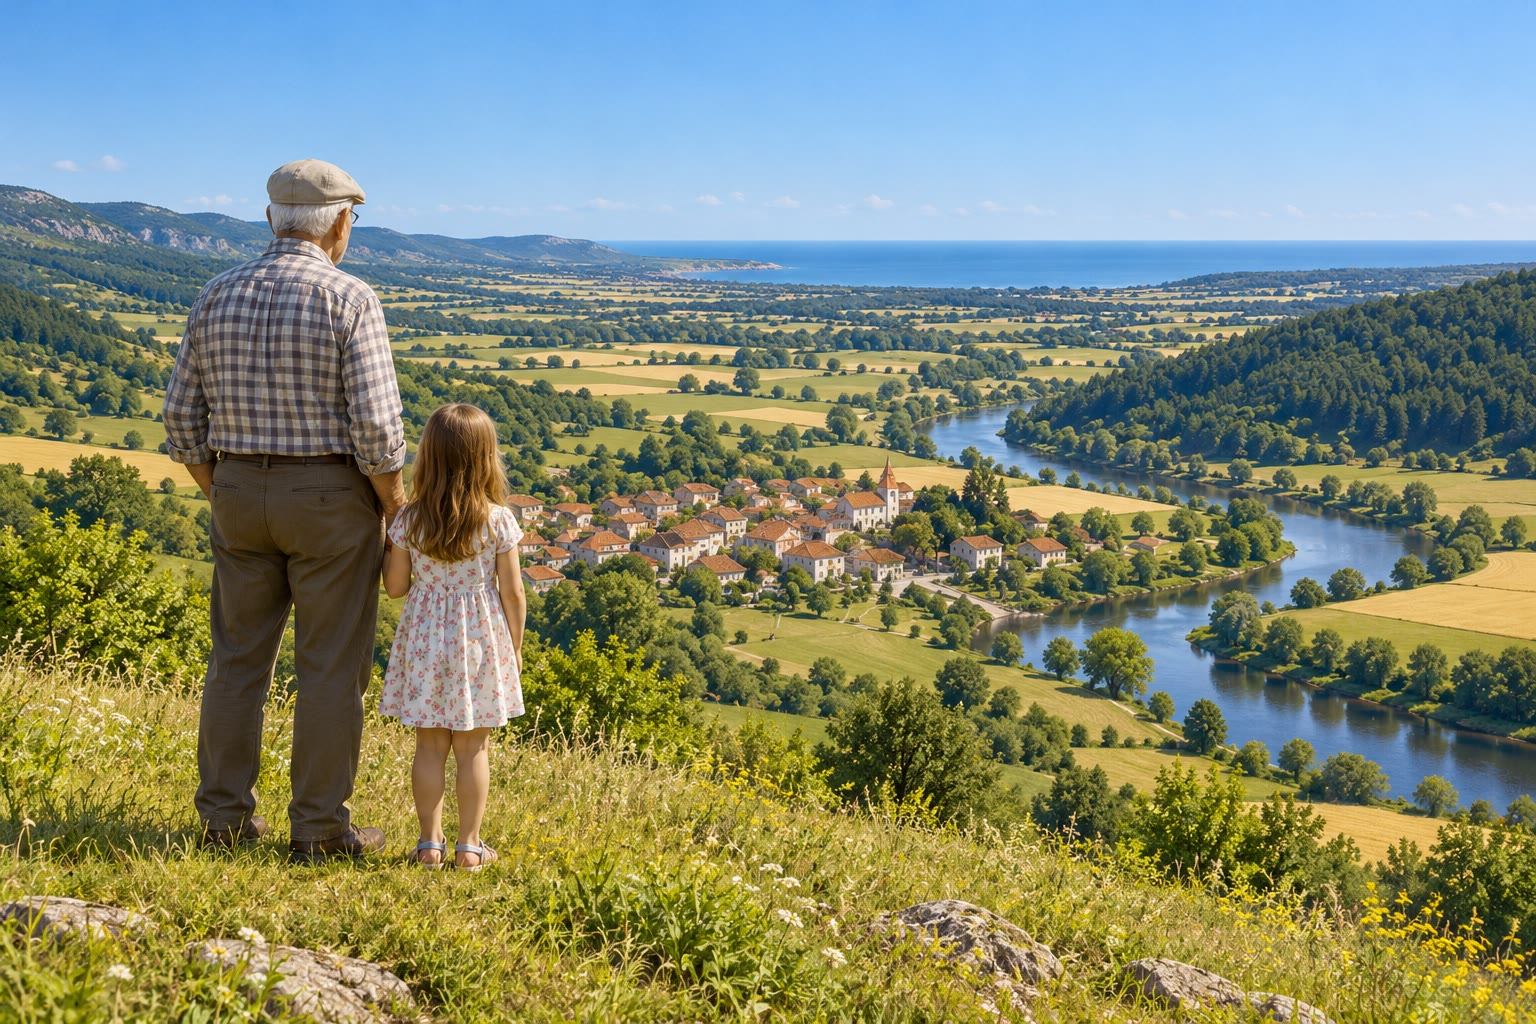
\includegraphics[width=0.72\linewidth]{images/book1/ai/g1-hilltop-view.jpg}

{\small Vanaf de top van een \omterm{def:g1:landscapes-around-us:landform}{heuvel} zien we een heel \omterm{def:g1:landscapes-around-us:landscape}{landschap}.}
\end{omfigure}

\section{Wat is een landschap?}

\begin{definition}[Landschap]\label{def:g1:landscapes-around-us:landscape}
Een \emph{landschap}\index{landschap} is alles wat we in één blik van het
land kunnen zien, van waar we staan tot aan de verre horizon: de vorm van
de grond, het water, de planten en de dingen die mensen hebben gebouwd.
\end{definition}

Een \omterm{def:g1:landscapes-around-us:landscape}{landschap} heeft delen die dichtbij zijn en delen die ver weg zijn. Het
deel dat het dichtst bij ons is, zit onderaan in wat we zien; het lijkt
groot en we zien er alle details van. Het verre deel zit bovenaan, vlak bij
de hemel; het lijkt klein en bleek.

\begin{omfigure}
\begin{tikzpicture}[x=1cm, y=1cm]
  \fill[ocBlue!12] (0,0) rectangle (10,5);
  % background: far hills
  \fill[black!18] (0,3.0) -- (1.5,3.6) -- (3,3.3) -- (5,3.9) -- (7,3.4) -- (8.5,3.8) -- (10,3.3) -- (10,2.9) -- (0,2.9) -- cycle;
  % middle: hills and fields
  \fill[green!35!omLithAlluv] (0,1.6) -- (2,2.4) -- (4,2.1) -- (6,2.7) -- (8,2.2) -- (10,2.5) -- (10,1.5) -- (0,1.5) -- cycle;
  \fill[green!25!omLithAlluv] (0,1.5) rectangle (10,2.95);
  \fill[green!35!omLithAlluv] (0,2.95) -- (2,3.1) -- (4,2.95) -- (6,3.25) -- (8,3.0) -- (10,3.1) -- (10,2.9) -- (0,2.9) -- cycle;
  \foreach \x in {5.6,5.9,6.2} \fill[red!55] (\x,2.25) -- ++(0.12,0.15) -- ++(0.12,-0.15) -- cycle;
  \foreach \x in {5.6,5.9,6.2} \fill[white] (\x+0.03,2.1) rectangle ++(0.18,0.15);
  % foreground
  \fill[green!55!black!60] (0,0) rectangle (10,1.5);
  \foreach \x in {0.8,2.1,8.6} {
    \fill[brown!70!black] (\x-0.06,0.4) rectangle (\x+0.06,0.9);
    \fill[green!45!black] (\x,1.15) circle (0.38);
  }
  % band borders and labels
  \draw[white, line width=1pt, dashed] (0,1.5) -- (10,1.5);
  \draw[white, line width=1pt, dashed] (0,2.95) -- (10,2.95);
  \node[font=\small\bfseries, fill=white, fill opacity=0.8, text opacity=1, inner sep=2pt] at (5,0.6) {voorgrond: dichtbij, groot, veel details};
  \node[font=\small\bfseries, fill=white, fill opacity=0.8, text opacity=1, inner sep=2pt] at (2.7,2.2) {middengrond};
  \node[font=\small\bfseries, fill=white, fill opacity=0.8, text opacity=1, inner sep=2pt] at (5,4.4) {achtergrond: ver, klein, bleek};
\end{tikzpicture}

{\small Een \omterm{def:g1:landscapes-around-us:landscape}{landschap} in drie stroken: de voorgrond onderaan, de
middengrond, en de achtergrond tegen de hemel.}
\label{fig:g1:landscapes-around-us:bands}
\end{omfigure}

\section{De vormen van het land}

De grond is niet overal vlak. Op sommige plaatsen rijst hij hoog op naar
de hemel; op andere zakt hij weg in lange laagten; elders is hij vlak
zover we kunnen kijken. Elke vorm krijgt een naam.

\begin{definition}[Landvormen]\label{def:g1:landscapes-around-us:landform}
Een \emph{landvorm}\index{landvorm} is een vorm van het oppervlak van het land.
\begin{itemize}
  \item Een \emph{berg}\index{berg} is een heel hoge landvorm met steile
        hellingen; zijn hoogste punt heet de top. Op de hoogste bergen
        ligt zelfs in de zomer sneeuw.
  \item Een \emph{heuvel}\index{heuvel} is een landvorm die boven het land
        eromheen uitsteekt, lager en ronder dan een berg.
  \item Een \emph{dal}\index{dal} is een lange, lage laagte tussen heuvels
        of bergen; onderin stroomt vaak een \omterm{def:g1:landscapes-around-us:water}{rivier}.
  \item Een \emph{vlakte}\index{vlakte} is een breed, vlak en laag stuk land.
\end{itemize}
\end{definition}

\begin{omfigure}
\begin{tikzpicture}[x=1cm, y=1cm]
  \fill[ocBlue!10] (0,0) rectangle (12.4,4.6);
  % sea
  \fill[omSea] (10.2,0) rectangle (12.4,0.55);
  % land profile: mountains, valley, hill, plain, coast
  \fill[omLithAlluv!80!green] (0,0) -- (0,2.2) -- (0.9,3.3) -- (1.5,3.0) -- (2.2,4.1)
     -- (2.9,2.6) -- (3.6,1.2) -- (3.9,0.9) -- (4.2,1.2) -- (5.0,2.0) -- (5.7,2.2)
     -- (6.4,1.6) -- (7.0,0.95) -- (8.0,0.8) -- (9.5,0.7) -- (10.2,0.6) -- (10.4,0.55)
     -- (10.4,0) -- cycle;
  \draw[black!60, line width=0.6pt] (0,2.2) -- (0.9,3.3) -- (1.5,3.0) -- (2.2,4.1)
     -- (2.9,2.6) -- (3.6,1.2) -- (3.9,0.9) -- (4.2,1.2) -- (5.0,2.0) -- (5.7,2.2)
     -- (6.4,1.6) -- (7.0,0.95) -- (8.0,0.8) -- (9.5,0.7) -- (10.2,0.6) -- (10.4,0.55);
  % snow caps
  \fill[white, draw=black!50, line width=0.3pt] (1.95,3.72) -- (2.2,4.1) -- (2.45,3.72) -- (2.3,3.78) -- (2.2,3.68) -- (2.08,3.78) -- cycle;
  \fill[white, draw=black!50, line width=0.3pt] (0.72,3.08) -- (0.9,3.3) -- (1.05,3.15) -- (0.9,3.12) -- cycle;
  % river in the valley
  \fill[omSea!90!black] (3.75,0.92) rectangle (4.05,0.98);
  % lake on the plain
  \fill[omSea] (7.6,0.82) ellipse (0.5 and 0.07);
  % village on the plain
  \foreach \x in {8.6,8.85,9.1} {
    \fill[white, draw=black!50, line width=0.3pt] (\x,0.74) rectangle ++(0.18,0.16);
    \fill[red!60] (\x-0.02,0.9) -- ++(0.11,0.12) -- ++(0.11,-0.12) -- cycle;
  }
  % labels
  \node[font=\small, above] at (2.2,4.12) {berg};
  \node[font=\small, above] at (5.6,2.25) {heuvel};
  \node[font=\small] at (3.9,1.85) {dal};
  \node[font=\small, above] at (8.2,1.5) {vlakte};
  \draw[black!60, thin] (8.2,1.5) -- (8.2,0.85);
  \node[font=\small, align=center] at (11.3,1.4) {zee};
  \node[font=\scriptsize, below=2pt, fill=white, fill opacity=0.8, text opacity=1, inner sep=1pt] at (7.6,0.35) {meer};
  \draw[black!60, thin] (7.6,0.45) -- (7.6,0.78);
  \node[font=\scriptsize, below=2pt, fill=white, fill opacity=0.8, text opacity=1, inner sep=1pt] at (10.3,0.35) {kust};
  \node[font=\scriptsize, fill=white, fill opacity=0.8, text opacity=1, inner sep=1pt] at (3.9,0.2) {rivier};
  \draw[black!60, thin] (3.9,0.32) -- (3.9,0.88);
\end{tikzpicture}

{\small De vormen van het land, van de \omterm{def:g1:landscapes-around-us:landform}{bergen} tot de zee, van opzij gezien
(de hoogten zijn veel hoger getekend dan ze in het echt zijn).}
\label{fig:g1:landscapes-around-us:profile}
\end{omfigure}

\begin{omfigure}
\begin{minipage}[b]{0.49\linewidth}\centering
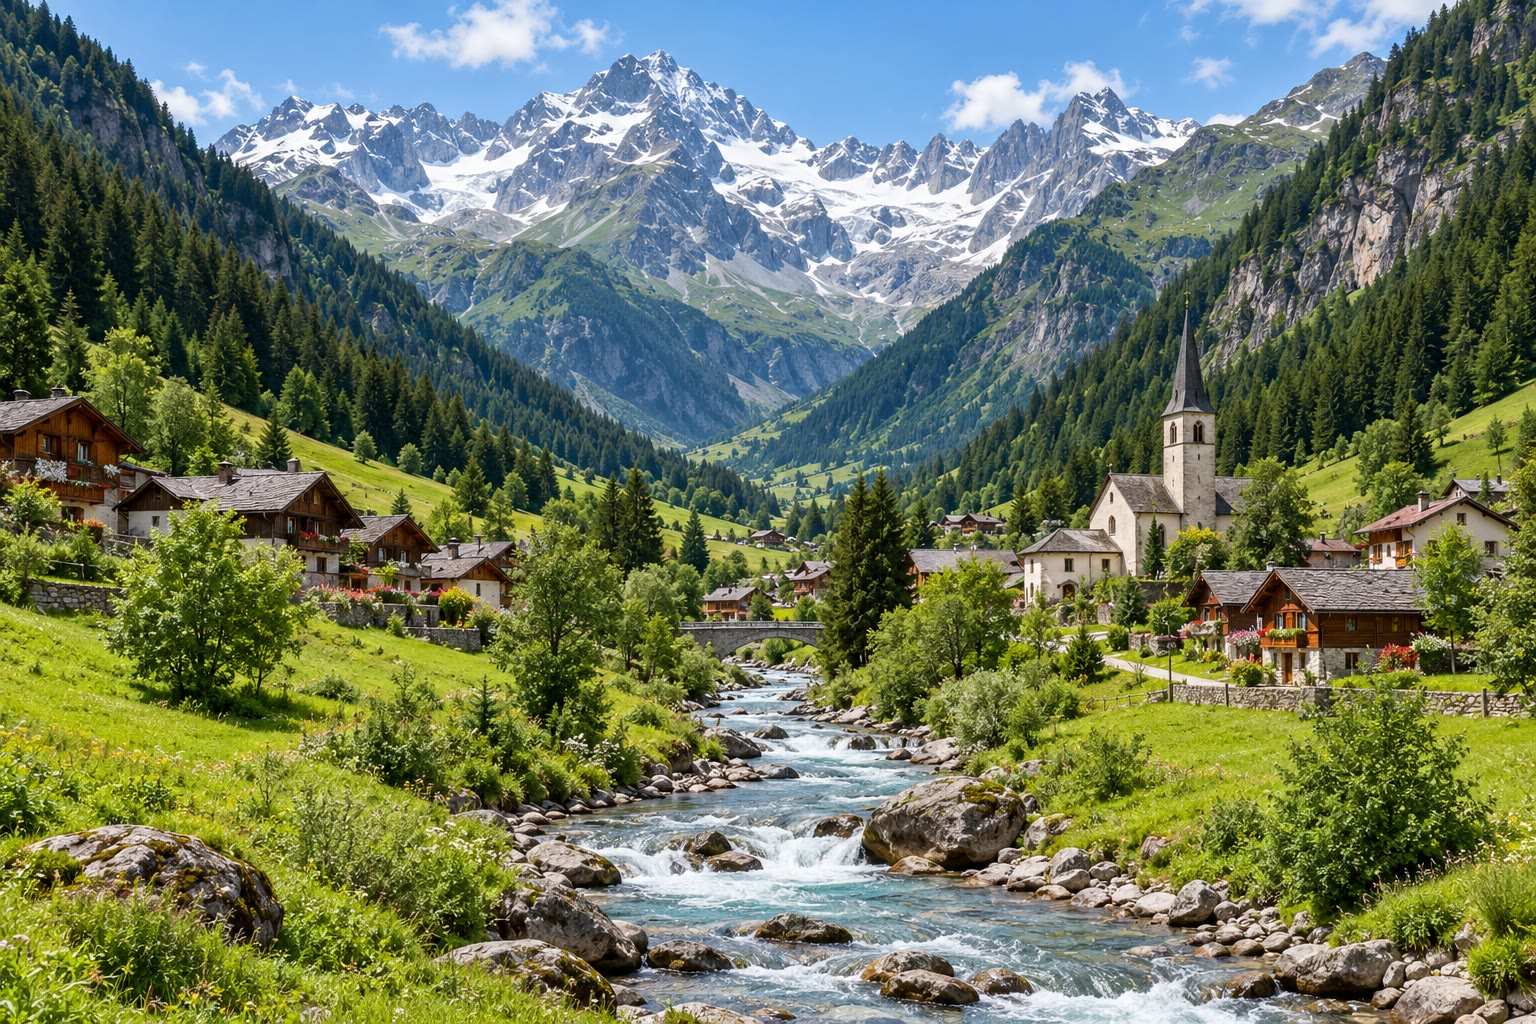
\includegraphics[width=\linewidth]{images/book1/ai/g1-mountain-village.jpg}

{\small \omterm{def:g1:landscapes-around-us:landform}{Bergen}, met een dorp in hun \omterm{def:g1:landscapes-around-us:landform}{dal}.}
\end{minipage}\hfill
\begin{minipage}[b]{0.49\linewidth}\centering
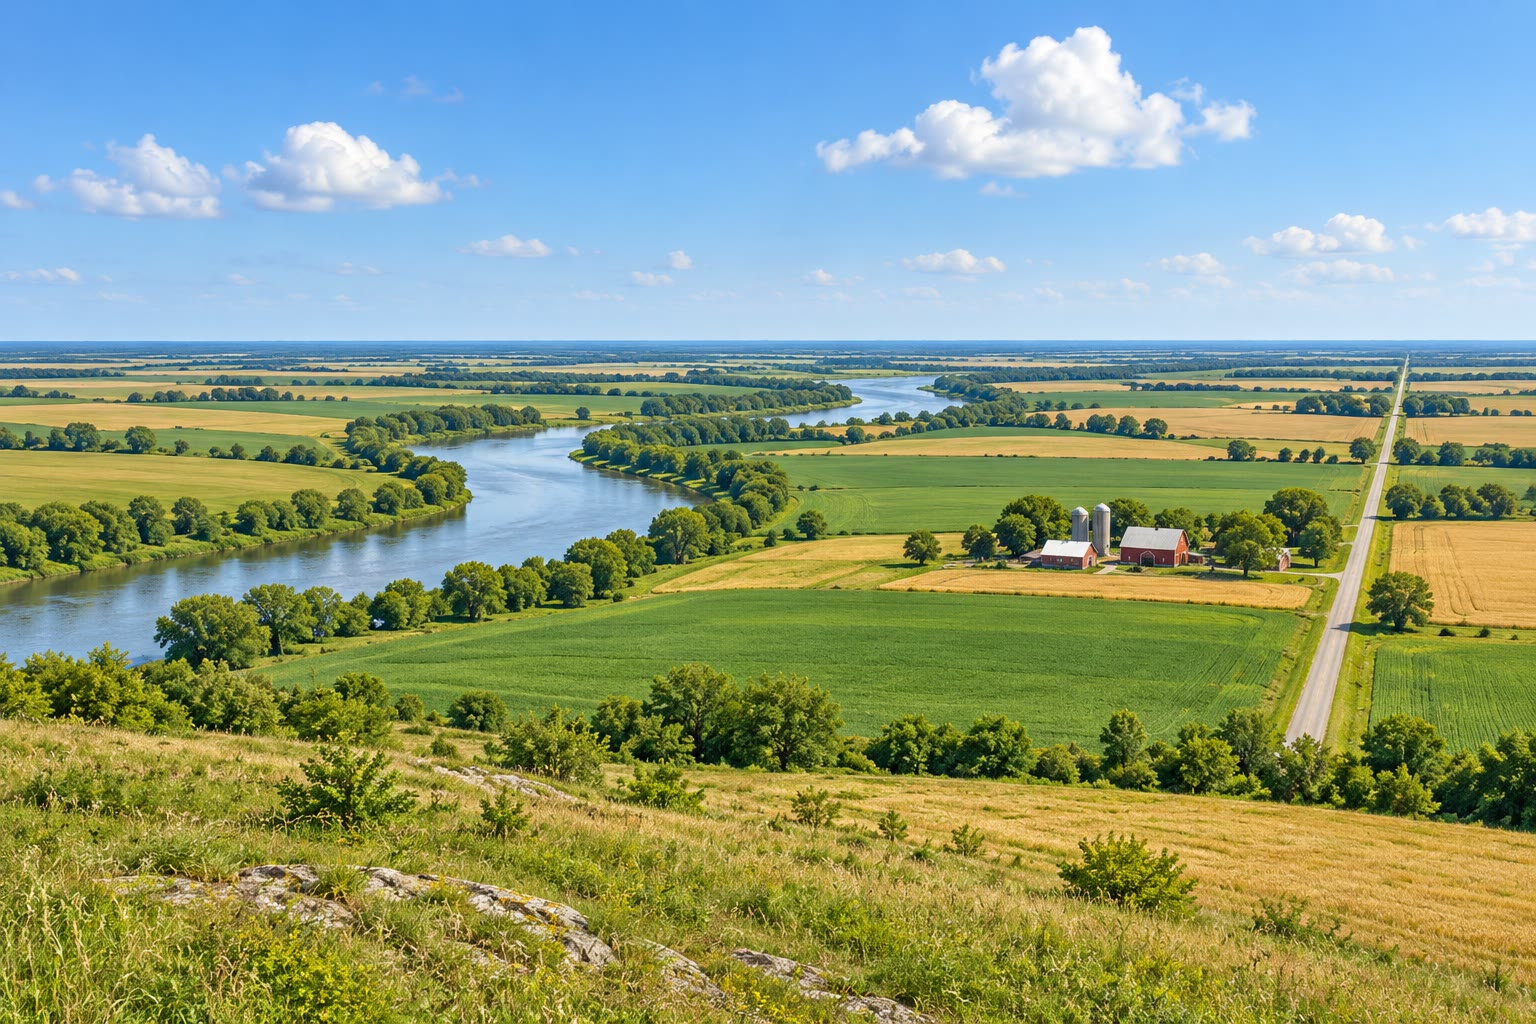
\includegraphics[width=\linewidth]{images/book1/ai/g1-plain-river.jpg}

{\small Een \omterm{def:g1:landscapes-around-us:landform}{vlakte}, met een \omterm{def:g1:landscapes-around-us:water}{rivier} en akkers.}
\end{minipage}
\end{omfigure}

\begin{example}[Berg of heuvel?]\label{ex:g1:landscapes-around-us:mountain-hill}
Er is geen precieze hoogte waarop een \omterm{def:g1:landscapes-around-us:landform}{heuvel} een \omterm{def:g1:landscapes-around-us:landform}{berg} wordt. We kijken naar
de vorm: een \omterm{def:g1:landscapes-around-us:landform}{berg} is hoog en steil, vaak rotsig, soms met sneeuw op de top;
een \omterm{def:g1:landscapes-around-us:landform}{heuvel} is lager en ronder, vaak begroeid met gras, akkers of bos, en we
kunnen in korte tijd naar zijn top lopen.
\end{example}

\section{Water in het landschap}

Water hoort bij de meeste \omterm{def:g1:landscapes-around-us:landscape}{landschappen}. Het stroomt van de \omterm{def:g1:landscapes-around-us:landform}{heuvels} en de
\omterm{def:g1:landscapes-around-us:landform}{bergen} naar beneden, verzamelt zich in laagten en bereikt de zee.

\begin{definition}[Water in een landschap]\label{def:g1:landscapes-around-us:water}
Een \emph{rivier}\index{rivier} is water dat altijd stroomt, in een lange
bedding, van hoger land naar beneden tot in een meer of in de zee. Een
\emph{meer}\index{meer} is een groot water met land eromheen. De
\emph{kust}\index{kust} is de plek waar het land de zee raakt.
\end{definition}

\begin{omfigure}
\begin{minipage}[b]{0.49\linewidth}\centering
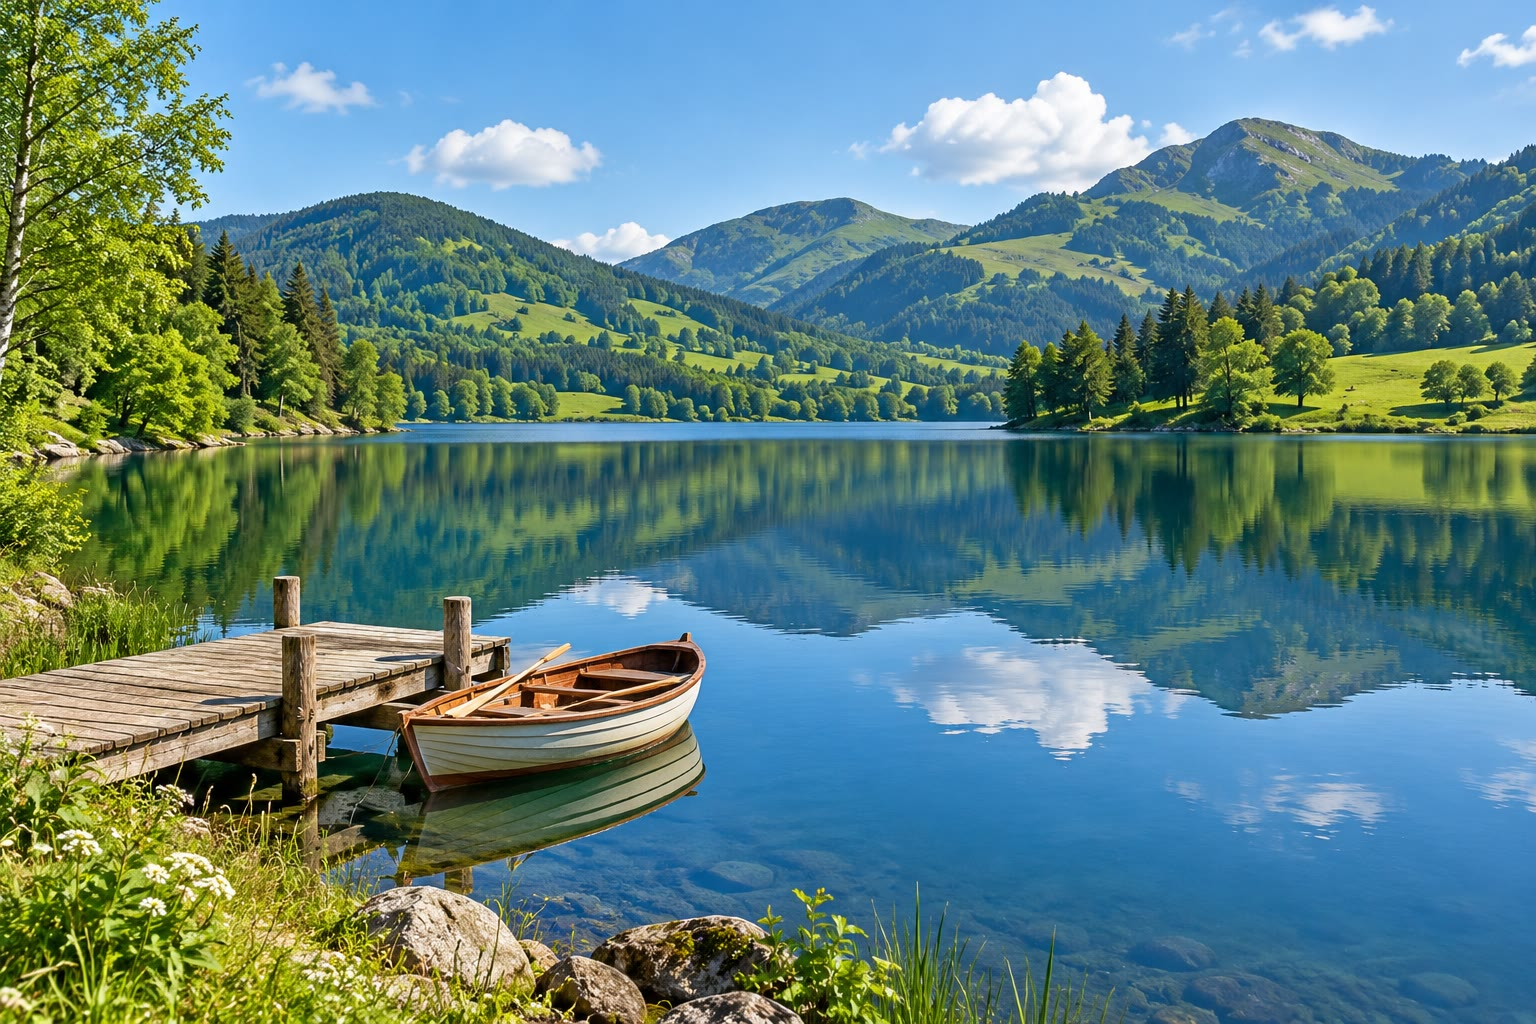
\includegraphics[width=\linewidth]{images/book1/ai/g1-lake-hills.jpg}

{\small Een \omterm{def:g1:landscapes-around-us:water}{meer} tussen \omterm{def:g1:landscapes-around-us:landform}{heuvels}.}
\end{minipage}\hfill
\begin{minipage}[b]{0.49\linewidth}\centering
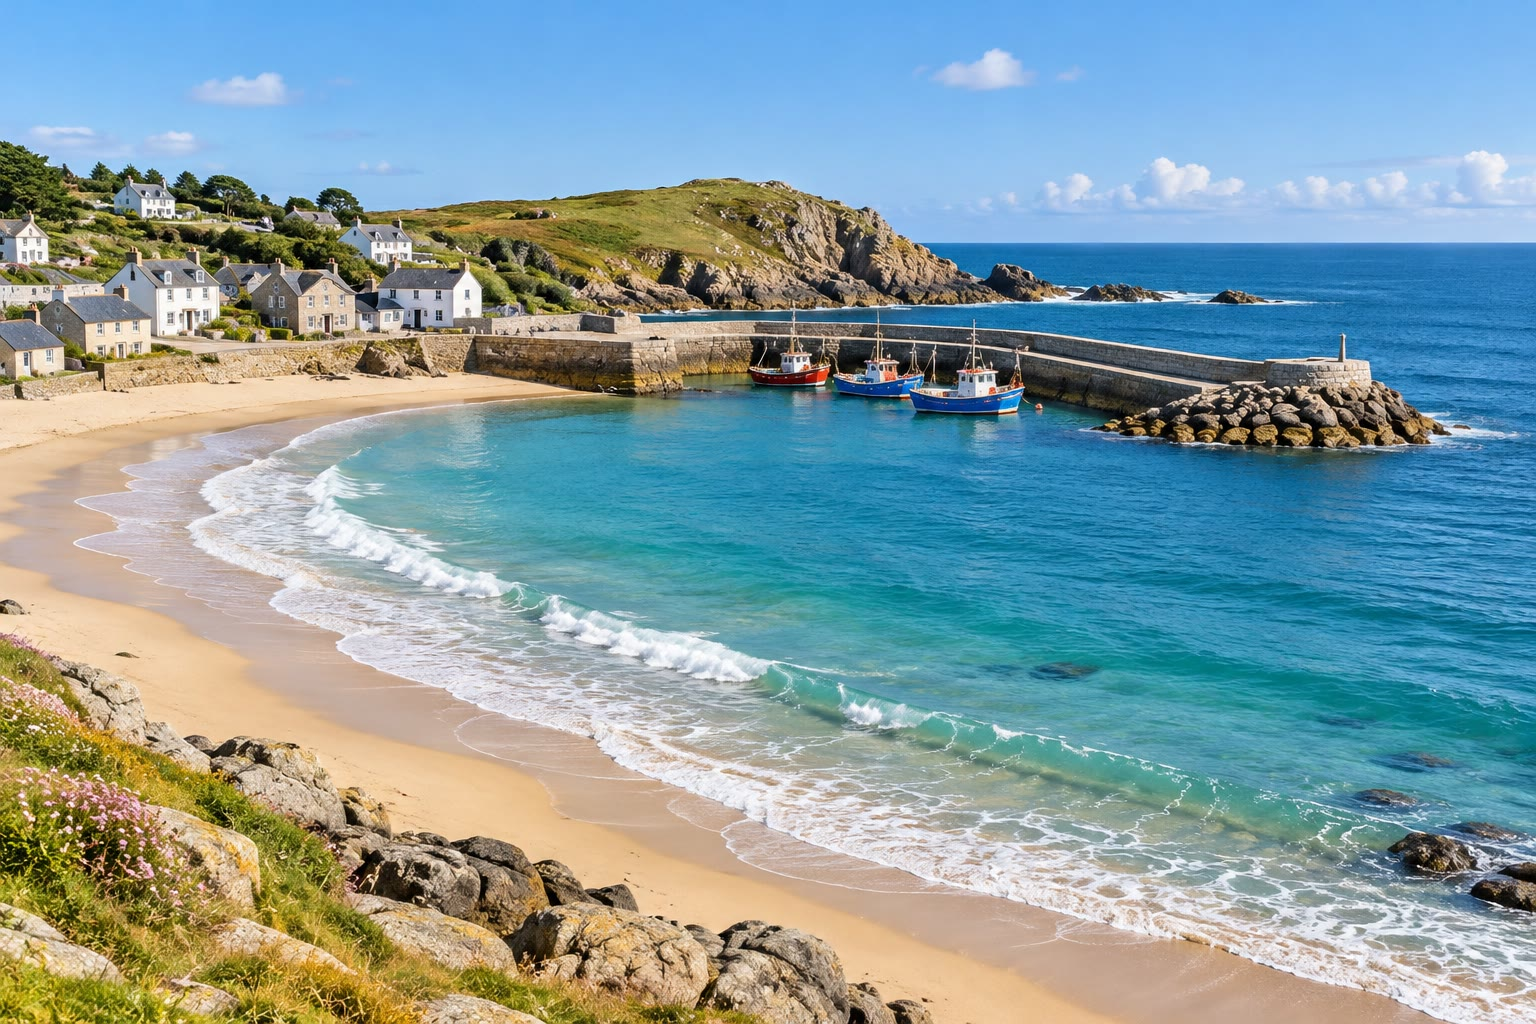
\includegraphics[width=\linewidth]{images/book1/ai/g1-coast-harbour.jpg}

{\small Een \omterm{def:g1:landscapes-around-us:water}{kust}: een strand, rotsen en een haven.}
\end{minipage}
\end{omfigure}

\begin{remark}[Water stroomt altijd naar beneden]\label{rem:g1:landscapes-around-us:downhill}
Een \omterm{def:g1:landscapes-around-us:water}{rivier} stroomt altijd van hoger naar lager gelegen grond. Daarom lopen
\omterm{def:g1:landscapes-around-us:water}{rivieren} onderin \omterm{def:g1:landscapes-around-us:landform}{dalen}, en daarom komen ze uiteindelijk in een \omterm{def:g1:landscapes-around-us:water}{meer} of in
de zee uit: die liggen lager dan het land eromheen.
\end{remark}

\section{Natuurlijke en door mensen gemaakte delen}

Sommige delen van een \omterm{def:g1:landscapes-around-us:landscape}{landschap} waren er al voordat er mensen kwamen: de
\omterm{def:g1:landscapes-around-us:landform}{bergen}, de \omterm{def:g1:landscapes-around-us:water}{rivieren}, de bossen. Andere delen zijn door mensen gemaakt:
huizen, wegen, bruggen, akkers.

\begin{definition}[Natuurlijke en door mensen gemaakte delen]\label{def:g1:landscapes-around-us:natural-built}
Een \emph{natuurlijk element}\index{natuurlijk element} van een \omterm{def:g1:landscapes-around-us:landscape}{landschap} is
een deel dat niet door mensen gemaakt is: een \omterm{def:g1:landscapes-around-us:landform}{berg}, een \omterm{def:g1:landscapes-around-us:water}{rivier}, een \omterm{def:g1:landscapes-around-us:water}{meer},
een bos, een strand. Een \emph{door mensen gemaakt
element}\index{door mensen gemaakt element} is een deel dat mensen
gemaakt of gevormd hebben: een huis, een weg, een
brug, een haven, een akker, een tuin.
\end{definition}

\begin{omfigure}
\begin{tikzpicture}[x=1cm, y=1cm]
  \node[draw=omDef!80!black, fill=omDef!10, rounded corners, text width=5.2cm,
        align=left, minimum height=3.2cm, anchor=north] (n) at (0,0)
    {\textbf{natuurlijk}\\[2pt] berg\\ heuvel\\ dal\\ rivier\\ meer\\ bos\\ strand};
  \node[draw=omMeth!80!black, fill=omMeth!10, rounded corners, text width=5.2cm,
        align=left, minimum height=3.2cm, anchor=north] (b) at (6,0)
    {\textbf{gemaakt door mensen}\\[2pt] huis\\ kerk\\ weg\\ brug\\ haven\\ akker\\ tuin};
\end{tikzpicture}

{\small De delen van het \omterm{def:g1:landscapes-around-us:landscape}{landschap} van Mia gesorteerd. Een akker is
door mensen gemaakt: ze hebben het land vrijgemaakt en er gewassen op geplant.}
\label{fig:g1:landscapes-around-us:sort}
\end{omfigure}

\section{Landschappen veranderen}

Een \omterm{def:g1:landscapes-around-us:landscape}{landschap} blijft niet voor altijd hetzelfde. Sommige veranderingen
gaan snel, andere zo langzaam dat niemand ze in een heel mensenleven ziet.
\begin{itemize}
  \item \textbf{Met de seizoenen:} de akkers zijn bruin na het ploegen,
        groen in de lente en goudgeel voor de oogst; de bomen verliezen hun
        bladeren in de herfst; in de winter kan sneeuw alles bedekken.
  \item \textbf{Door de mensen:} een dorp groeit uit tot een stad; een bos
        wordt gekapt om er akkers van te maken; een nieuwe weg en een brug
        gaan over het \omterm{def:g1:landscapes-around-us:landform}{dal}.
  \item \textbf{Door water en weer:} na een zware storm kan een \omterm{def:g1:landscapes-around-us:water}{rivier}
        buiten haar oevers treden en een paar dagen de akkers bedekken; aan
        de \omterm{def:g1:landscapes-around-us:water}{kust} slijten de golven de rotsen langzaam weg.
\end{itemize}

\begin{omfigure}
\begin{tikzpicture}[x=1cm, y=1cm]
  \foreach \k/\t in {0/lang geleden, 1/vandaag} {
  \begin{scope}[shift={(\k*6.4,0)}]
    \fill[ocBlue!8] (0,0) rectangle (5.8,3.4);
    \fill[green!30!omLithAlluv] (0,0) rectangle (5.8,1.9);
    % river
    \fill[omSea] (0,0.55) .. controls (1.5,0.9) and (2.5,0.2) .. (5.8,0.6)
       -- (5.8,0.85) .. controls (2.5,0.45) and (1.5,1.15) .. (0,0.8) -- cycle;
    % hill
    \fill[green!45!black!55] (2.8,1.9) .. controls (3.8,3.1) and (4.8,3.1) .. (5.8,2.2) -- (5.8,1.9) -- cycle;
    \ifnum\k=0
      % forest everywhere, a few houses
      \foreach \x in {0.4,0.9,1.4,1.9,2.4,4.3,4.8,5.3}
        \fill[green!40!black] (\x,1.45) circle (0.22);
      \foreach \x in {3.4,3.75} {
        \fill[white, draw=black!50, line width=0.3pt] (\x,1.15) rectangle ++(0.24,0.2);
        \fill[red!60] (\x-0.03,1.35) -- ++(0.15,0.14) -- ++(0.15,-0.14) -- cycle; }
    \else
      % fields, many houses, a road and a bridge
      \foreach \x/\c in {0.1/yellow!60, 1.3/green!55, 4.5/yellow!45}
        \fill[\c] (\x,1.05) rectangle ++(1.1,0.5);
      \fill[black!35] (2.65,0) rectangle (2.95,1.9);
      \fill[black!55] (2.55,0.5) rectangle (3.05,0.9);
      \foreach \x in {3.2,3.55,3.9} \foreach \y in {1.1,1.45} {
        \fill[white, draw=black!50, line width=0.3pt] (\x,\y) rectangle ++(0.24,0.2);
        \fill[red!60] (\x-0.03,\y+0.2) -- ++(0.15,0.14) -- ++(0.15,-0.14) -- cycle; }
      \foreach \x in {4.6,5.2} \fill[green!40!black] (\x,2.35) circle (0.2);
    \fi
    \node[font=\small\bfseries] at (2.9,-0.3) {\t};
  \end{scope}}
\end{tikzpicture}

{\small Hetzelfde \omterm{def:g1:landscapes-around-us:landform}{dal} lang geleden en vandaag. De \omterm{def:g1:landscapes-around-us:landform}{heuvel} en de \omterm{def:g1:landscapes-around-us:water}{rivier} zijn
niet verplaatst; de mensen hebben het grootste deel van het bos gekapt,
akkers aangelegd en meer huizen, een weg en een brug gebouwd.}
\label{fig:g1:landscapes-around-us:change}
\end{omfigure}

\begin{example}[Stad en platteland]\label{ex:g1:landscapes-around-us:town}
In een stad is bijna alles wat we zien gebouwd: straten, huizen, winkels,
bruggen, parken. Op het platteland zien we vooral akkers, bossen en
weilanden, met hier en daar een boerderij of een dorp. Allebei zijn het
\omterm{def:g1:landscapes-around-us:landscape}{landschappen}. Zelfs midden in een grote stad zijn de vormen van het land
er nog: een \omterm{def:g1:landscapes-around-us:water}{rivier} stroomt door de stad, en sommige straten gaan een
\omterm{def:g1:landscapes-around-us:landform}{heuvel} op.
\end{example}

\section{Een landschap beschrijven}

\begin{method}[Een landschap beschrijven in vier stappen]\label{met:g1:landscapes-around-us:describe}
Zo beschrijf je een \omterm{def:g1:landscapes-around-us:landscape}{landschap}, vanaf een heuveltop of op een plaatje:
\begin{enumerate}
  \item \textbf{Verdeel het in drie stroken:} de voorgrond, de middengrond
        en de achtergrond.
  \item \textbf{Noem de vormen van het land:} \omterm{def:g1:landscapes-around-us:landform}{bergen}, \omterm{def:g1:landscapes-around-us:landform}{heuvels}, \omterm{def:g1:landscapes-around-us:landform}{dalen},
        \omterm{def:g1:landscapes-around-us:landform}{vlakten}.
  \item \textbf{Zoek het water:} een \omterm{def:g1:landscapes-around-us:water}{rivier}, een \omterm{def:g1:landscapes-around-us:water}{meer}, de zee en haar \omterm{def:g1:landscapes-around-us:water}{kust}.
  \item \textbf{Zoek wat mensen hebben gemaakt:} huizen, wegen, bruggen,
        akkers.
\end{enumerate}
\end{method}

\begin{example}[Het landschap van Mia]\label{ex:g1:landscapes-around-us:mia}
Op de voorgrond: het gras boven op de \omterm{def:g1:landscapes-around-us:landform}{heuvel}. Op de middengrond: een \omterm{def:g1:landscapes-around-us:landform}{dal}
met een \omterm{def:g1:landscapes-around-us:water}{rivier}, een brug en een dorp, met akkers eromheen, en een bos op de
volgende \omterm{def:g1:landscapes-around-us:landform}{heuvel}. Op de achtergrond: een \omterm{def:g1:landscapes-around-us:landform}{vlakte} en, aan het eind van het
land, de \omterm{def:g1:landscapes-around-us:water}{kust} en de zee. Natuurlijk: de \omterm{def:g1:landscapes-around-us:landform}{heuvels}, het \omterm{def:g1:landscapes-around-us:landform}{dal}, de \omterm{def:g1:landscapes-around-us:water}{rivier}, het
bos, de zee. Door mensen gemaakt: het dorp, de kerk, de brug, de akkers.
\end{example}

\section{Oefeningen}

\begin{exercise}[$\star$]\label{exo:g1:landscapes-around-us:1}
Noem de vier vormen van het land die je in dit hoofdstuk hebt geleerd.
\end{exercise}

\begin{exercise}[$\star$]\label{exo:g1:landscapes-around-us:2}
Wat is hoger en steiler: een \omterm{def:g1:landscapes-around-us:landform}{heuvel} of een \omterm{def:g1:landscapes-around-us:landform}{berg}?
\end{exercise}

\begin{exercise}[$\star$]\label{exo:g1:landscapes-around-us:3}
Natuurlijk of door mensen gemaakt? Een \omterm{def:g1:landscapes-around-us:water}{rivier}; een weg; een bos; een brug; een strand; een huis.
\end{exercise}

\begin{exercise}[$\star$]\label{exo:g1:landscapes-around-us:4}
Waar is de \omterm{def:g1:landscapes-around-us:water}{kust}: waar het land een \omterm{def:g1:landscapes-around-us:water}{rivier} raakt, of waar het land de zee
raakt?
\end{exercise}

\begin{exercise}[$\star$]\label{exo:g1:landscapes-around-us:5}
Kijk naar het plaatje van de \omterm{def:g1:landscapes-around-us:landform}{bergen} met hun dorp. Noem één \omterm{def:g1:landscapes-around-us:natural-built}{natuurlijk
element} en één \omterm{def:g1:landscapes-around-us:natural-built}{door mensen gemaakt element}.
\end{exercise}

\begin{exercise}[$\star$]\label{exo:g1:landscapes-around-us:6}
Welke \omterm{def:g1:landscapes-around-us:landform}{landvorm} is op de tekening van de vormen van het land het hoogst?
Waar stroomt de \omterm{def:g1:landscapes-around-us:water}{rivier}?
\end{exercise}

\begin{exercise}[$\star\star$]\label{exo:g1:landscapes-around-us:7}
Waar komt een \omterm{def:g1:landscapes-around-us:water}{rivier} vandaan, en waar gaat ze naartoe? Waarom stroomt ze
nooit omhoog naar de top van een \omterm{def:g1:landscapes-around-us:landform}{heuvel}?
\end{exercise}

\begin{exercise}[$\star\star$]\label{exo:g1:landscapes-around-us:8}
Op een plaatje van een \omterm{def:g1:landscapes-around-us:landscape}{landschap} lijkt een boom onderaan groter dan een
hele \omterm{def:g1:landscapes-around-us:landform}{heuvel} bovenaan. Hoe komt dat?
\end{exercise}

\begin{exercise}[$\star\star$]\label{exo:g1:landscapes-around-us:9}
Beschrijf het plaatje van de \omterm{def:g1:landscapes-around-us:landform}{vlakte} met haar \omterm{def:g1:landscapes-around-us:water}{rivier} in drie stroken: wat
staat er op de voorgrond, op de middengrond en op de achtergrond?
\end{exercise}

\begin{exercise}[$\star\star$]\label{exo:g1:landscapes-around-us:10}
Een tarweveld is groen of goudgeel, net als gras. Waarom zeggen we dat het
een \omterm{def:g1:landscapes-around-us:natural-built}{door mensen gemaakt element} van het \omterm{def:g1:landscapes-around-us:landscape}{landschap} is en geen \omterm{def:g1:landscapes-around-us:natural-built}{natuurlijk
element}?
\end{exercise}

\begin{exercise}[$\star\star$]\label{exo:g1:landscapes-around-us:11}
Kijk naar de tekening van het \omterm{def:g1:landscapes-around-us:landform}{dal} lang geleden en vandaag. Noem twee
dingen die niet veranderd zijn en drie dingen die mensen hebben toegevoegd.
\end{exercise}
